\documentclass[sigconf]{acmart}

\usepackage{booktabs} % For formal tables
\usepackage{graphicx}
\usepackage{balance}  % for  \balance command ON LAST PAGE  (only there!)
\usepackage{amssymb}
\usepackage{graphicx}
\usepackage{float}
\usepackage{subfigure}
\usepackage{mathtools}
\usepackage{eurosym}

\usepackage{pgfplots}
\usepackage{url}
\usepackage{enumitem}
\usepackage[linesnumbered,ruled]{algorithm2e}
\usepackage[export]{adjustbox}
\usepackage{xspace}
\usepackage{breqn}

% Copyright
%\setcopyright{none}
%\setcopyright{acmcopyright}
%\setcopyright{acmlicensed}
\setcopyright{rightsretained}
%\setcopyright{usgov}
%\setcopyright{usgovmixed}
%\setcopyright{cagov}
%\setcopyright{cagovmixed}


% DOI
\acmDOI{10.475/XXX_X}

% ISBN
\acmISBN{XXX-XXX-XX-XXX/10/18}

%Conference
\acmConference[CIKM'18]{ACM International Conference on Information and Knowledge Management}{October 2018}{
  Lingotto, Turin Italy}
\acmYear{2018}
\copyrightyear{2018}


\acmArticle{4}
\acmPrice{15.00}

% These commands are optional
%\acmBooktitle{Transactions of the ACM Woodstock conference}
\editor{Rakesh Agrawal}
\editor{Andrei Broder}
\editor{Mohammed Zaki}


\begin{document}
\title{Exploration of Interesting Dense Regions on Spatial Data}
%\titlenote{Produces the permission block, and
%  copyright information}
%\subtitle{Extended Abstract}
%\subtitlenote{The full version of the author's guide is available as
%  \texttt{acmart.pdf} document}

\author{Double-blind submission}

% \author{Behrooz Omidvar-Tehrani}
%\affiliation{%
  %\institution{University of Grenoble Alpes (France)}
%}
%\email{behrooz.omidvar-tehrani@univ-grenoble-alpes.fr}

%\author{Pl\'acido A. Souza Neto}
%\affiliation{%
 % \institution{Federal Institute of Rio Grande do Norte (Brazil)}
%}
%\email{placido.neto@ifrn.edu.br}


%\author{Francisco B. Silva J\'unior}
%\affiliation{%
%\institution{Federal Institute of Rio Grande do Norte (Brazil)}
%}
%\email{bento.francisco@academico.ifrn.edu.br}	

%\author{Felipe F. Pontes}
%\affiliation{%
%\institution{Federal Institute of Rio Grande do Norte (Brazil)}
%}
%\email{freire.pontes@academico.ifrn.edu.br}


%\author{Tiago Oliveira Lisboa}
%\affiliation{%
% \institution{Federal Institute of Rio Grande do Norte (Brazil)}
%}
%\email{tiago.oliveira@academico.ifrn.edu.br}



% The default list of authors is too long for headers.
%\renewcommand{\shortauthors}{B. Trovato et al.}


\begin{abstract}
The large size of spatial data hinders its effective analysis for insight discovery. Analysts require to obtain few high quality options (i.e., ``highlights'') to have a more focused investigation. In this paper, we define, formalize and analyze Interesting Dense Regions (IDRs) which capture implicit preferences of analysts in order to automatically find highlights. Our approach involves a polygon-based abstraction layer for captured preferences. Using these interesting dense regions, we highlight points to guide the analysis process. We analyze the efficiency and effectiveness of our approach through a realistic example.
\end{abstract}

%
% The code below should be generated by the tool at
% http://dl.acm.org/ccs.cfm
% Please copy and paste the code instead of the example below.
%
%\begin{CCSXML}
%<ccs2012>
 %<concept>
  %<concept_id>10010520.10010553.10010562</concept_id>
  %<concept_desc>Computer systems organization~Embedded systems</concept_desc>
  %<concept_significance>500</concept_significance>
 %</concept>
 %<concept>
  %<concept_id>10010520.10010575.10010755</concept_id>
  %<concept_desc>Computer systems organization~Redundancy</concept_desc>
  %<concept_significance>300</concept_significance>
 %</concept>
 %<concept>
  %<concept_id>10010520.10010553.10010554</concept_id>
  %<concept_desc>Computer systems organization~Robotics</concept_desc>
  %<concept_significance>100</concept_significance>
 %</concept>
 %<concept>
 % <concept_id>10003033.10003083.10003095</concept_id>
  %<concept_desc>Networks~Network reliability</concept_desc>
  %<concept_significance>100</concept_significance>
 %</concept>
%</ccs2012>
%\end{CCSXML}

%\ccsdesc[500]{Computer systems organization~Embedded systems}
%\ccsdesc[300]{Computer systems organization~Redundancy}
%\ccsdesc{Computer systems organization~Robotics}
%\ccsdesc[100]{Networks~Network reliability}


\keywords{Spatial data, Implicit feedback, Dense regions, Spatial highlights.}


\maketitle



\section{Introduction}

Spatial data are often voluminous. Hence the focus in the literature of spatial data analysis is often on ``efficiency'', i.e., enabling fluid means of navigation in spatial data in order to facilitate the exploratory analysis. The common approach is to design pre-computed indexes which enable efficient retrieval of spatial data (e.g., \cite{lins2013nanocubes}). However, there has been fewer attention to the ``value'' derived from spatial data. Despite the huge progress on the efficiency front, an analyst may easily get lost in the plethora of geographical points due to two following reasons.

\begin{itemize}[leftmargin=*]
\setlength\itemsep{2pt}
\item In an exploratory context, the analyst doesn't know apriori what to investigate next.
\item Moreover, she may easily get distracted and miss interesting points by visual clutter caused by huge point overlaps.
\end{itemize}

\vspace{2pt}
The main drawback of the traditional analysis model (e.g.,~\cite{kamat2014distributed,Omidvar-Tehrani:2015,omidvar2017geoguide}, to name a few) is that the analyst has a {\em passive role} in the process. In other words, the analyst's feedback (i.e., her likes and dislikes) is ignored and only the input query (i.e., her explicit request) is served. In case feedback is incorporated, the process can be more directed towards analyst's interests where her partial needs can be served earlier in the process. In this paper, we advocate for a ``guidance layer'' on top of the raw visualization of spatial data to enable analysts know {\em ``what to see next''}. This guidance should be a function of analyst feedback: the system should recommend options similar to what the analyst has already appreciated. 
 
\vspace{2pt}
Considering this context, we propose in this paper an approach to explore Interesting Dense Regions (IDRs)  whose aim is to capture and analyze implicit feedback of analysts in spatial data analysis. Without loss of generality, we focus on ``mouse moves'' as the implicit feedback received from the analyst. Mouse moves are the most common way that analysts interact with geographical maps~\cite{Chen:2001}.  However, our approach can be easily extended to other types of inputs such gaze tracking~\cite{arapakis2014user} and leap motions.

% K-DBSCAN with the main focus of identifying clusters of points with similar spatial density.  K-DBSCAN lies in finding arbitrary shaped clusters in variable density regions. Moreover, it can also discover clusters with overlapping spatial regions, but differing density levels.
 
 
\section{Interesting Dense Regions}
An Interesting Dense Region (IDR) is a spatial region with high probability of having spatial points with potential interest to the analyst. An IDR is captured and defined by processing user feedbacks. Unlike the literature which mainly focuses on explicit refections, we investigate on implicit feedback. There are different ways to capture implicit feedbacks.

\begin{itemize}[leftmargin=*]
\setlength\itemsep{2pt}
\item During spatial data analysis, it is often the case that analysts look at some regions of interest but forget to provide an explicit feedback. We call this latent signal, gaze. It shown in~\cite{arapakis2014user} that gaze has a strong correlation with ``user attention''. The signal can be captured by tracking eye movements.
\item To address privacy issues of gaze exploitation, we consider an alternative option, i.e., tracking the mouse cursor. It is shown in \cite{arapakis2014understanding} that mouse gestures have a strong correlation with ``user engagement''. Intuitively, a point receives a positive feedback if the cursor moves around it frequently.
\end{itemize}

\vspace{2pt}
The objective of discovering IDRs is to obtain the preferences of analysts which have never been expressed explicitly. For such discovery, we are inspired by two observations.

\vspace{2pt}
\noindent $\blacksquare$ {\bf Observation 1.} We believe that a region appeals more interesting to the analyst if it is denser, i.e., the analyst moves her mouse in that region several times.

\vspace{2pt}
\noindent $\blacksquare$ {\bf Observation 2.} It is possible that the analyst moves her mouse everywhere in the map. This should not signify that everywhere in the map has the same significance.

\vspace{2pt}
We consider two different layers on a geographical map: ``spatial layer'' and ``interaction layer''. The spatial layer contains points from a spatial database $\mathcal{P}$. The interaction layer contains mouse move points $\mathcal{M}$. Our proposed approach mines a set of mouse move points $\mathcal{M}$ in the interaction layer to discover one or several IDRs, in which most analyst's interactions occur. Then it matches the spatial points $\mathcal{P}$ with IDRs in order to find points inside each region. We employ a Quadtree index as a mediator between the spatial and interaction layer in order to reduce the number of matchings. The attributes of resulting points will be exploited to update analyst's feedback vector $F$. The updated vector $F$ will then be used to find $k$ highlights (where $k$ is specified by the analyst). These steps ensure that the final highlights reflect analyst's implicit interests. 

\vspace{2pt}
Algorithm \ref{algo:dense} summarizes our approach for mining IDRs. We add points to $\mathcal{M}$ only every $200ms$ to prevent adding redundant points.  Following Observation 1 and in order to mine the recurring behavior of the analyst, the algorithm begins by partitioning the set $\mathcal{M}$ into $g$ fixed-length consecutive segments $\mathcal{M}_0$ to $\mathcal{M}_g$. The first segment starts at time zero (where the system started), and the last segment ends at $t_c$, i.e., the current time. Following Observation 2, we then find dense clusters in each segment of $\mathcal{M}$ using a variant of DB-SCAN approach~\cite{Ester:1996}. Finally, we return intersections among those clusters as IDRs.

\begin{algorithm}[t]
\DontPrintSemicolon
\KwIn{Current time $t_c$, mouse move points $\mathcal{M}$, number of highlights $k$}
\KwOut{$k$ highlights $\mathcal{H}$}
$\mathcal{S} \gets \emptyset$\;
$g \gets ${\em number of time segments}\;
\For{$i \in [0,g]$}
{
       $\mathcal{M}_i \gets \{m = \langle x,y,t \rangle | (\frac{t_c}{g} \times i) \leq t \leq (\frac{t_c}{g} \times (i+1))\}$\;
       $\mathcal{C}_i \gets \mathit{mine\_clusters}(\mathcal{M}_i)$\label{ln:mine}\;
       $\mathcal{O}_i \gets \mathit{find\_ploygons}(\mathcal{C}_i)$\label{ln:poly}\;
}
\lFor{$\mathcal{O}_i, \mathcal{O}_j$ where $i,j \in [0,g]$ and $i \neq j$}
{
       $\mathcal{S}.\mathit{append}(\mathit{intersect}(\mathcal{O}_i, \mathcal{O}_j))$
}
$\mathcal{H} \gets \mathit{discover\_highlights}(\mathcal{S},k)$\;
\Return{$\mathcal{H}$}\; 
\caption{Information Highlighting}
\label{algo:dense}
\end{algorithm}

\vspace{2pt}
For clustering points in each time segment (i.e., line \ref{ln:mine} of Algorithm~\ref{algo:dense}), we use ST-DBSCAN, a space-aware variant of DB-SCAN for clustering points based on density~\cite{Birant:2007}. For each subset of mouse move points $\mathcal{M}_i$, $i \in [0,g]$, ST-DBSCAN begins with a random point $m_0 \in \mathcal{M}_i$ and collects all density-reachable points from $m_0$ using a distance metric. As mouse move points occur in the 2-dimensional pixel space (i.e., the display), we choose euclidean distance as our metric. If $m_0$ turns out to be a core object, a cluster will be generated. Otherwise, if $m_0$ is a border object, no point is density-reachable from $m_0$ and the algorithm picks another random point in $\mathcal{M}_i$. The process is repeated until all of the points have been processed.

\vspace{2pt}
Once clusters are obtained for all subsets of $\mathcal{M}$, we find their intersections to locate recurring regions (line \ref{ln:poly}). To obtain intersections, we need to clearly define the spatial boundaries of each cluster. Hence for each cluster, we discover its corresponding polygon that covers the points inside. For this aim, we employ Quickhull algorithm, a quicksort-style method which computes the convex hull for a given set of points in a 2D plane~\cite{Barber:1996}.

\vspace{2pt}
There exist several approaches to infer a spatial region for a given set of points \cite{Bevis1989,DUCKHAM2008,FADILI2004,ARAMPATZIS2006,Galton2006}. The common approach is to cluster points in form of concave and convex polygons.  In case a concave polygon is constructed, the ``dents'' of such a polygon may entail points which are not necessarily in $\mathcal{M}$. In IDR algorithm, however, we adapt Quickhull~\cite{Barber:1996}, due its simplicity, efficiency and it's natural implementation of convex polygons.

\vspace{2pt}
Once the IDRs are discovered, we employ {\sc GeoGuide}, an algorithm proposed in \cite{omidvar2017geoguide}, to highlight $k$ points among the set of points inside IDRs. We seek two properties in $k$ highlights, i.e., {\em similarity} and {\em diversity}. First, highlights should be in the same direction of the analyst's implicit feedback, hence similar to the vector~$F$. Second, highlighted points should also represent distinct directions so that the analyst can observe different aspects of data and decide based on the big picture.

\section{Case Study}
We discuss a real-world example to show the functionality of our approach in practice.

\begin{figure*}[t]
\centering
   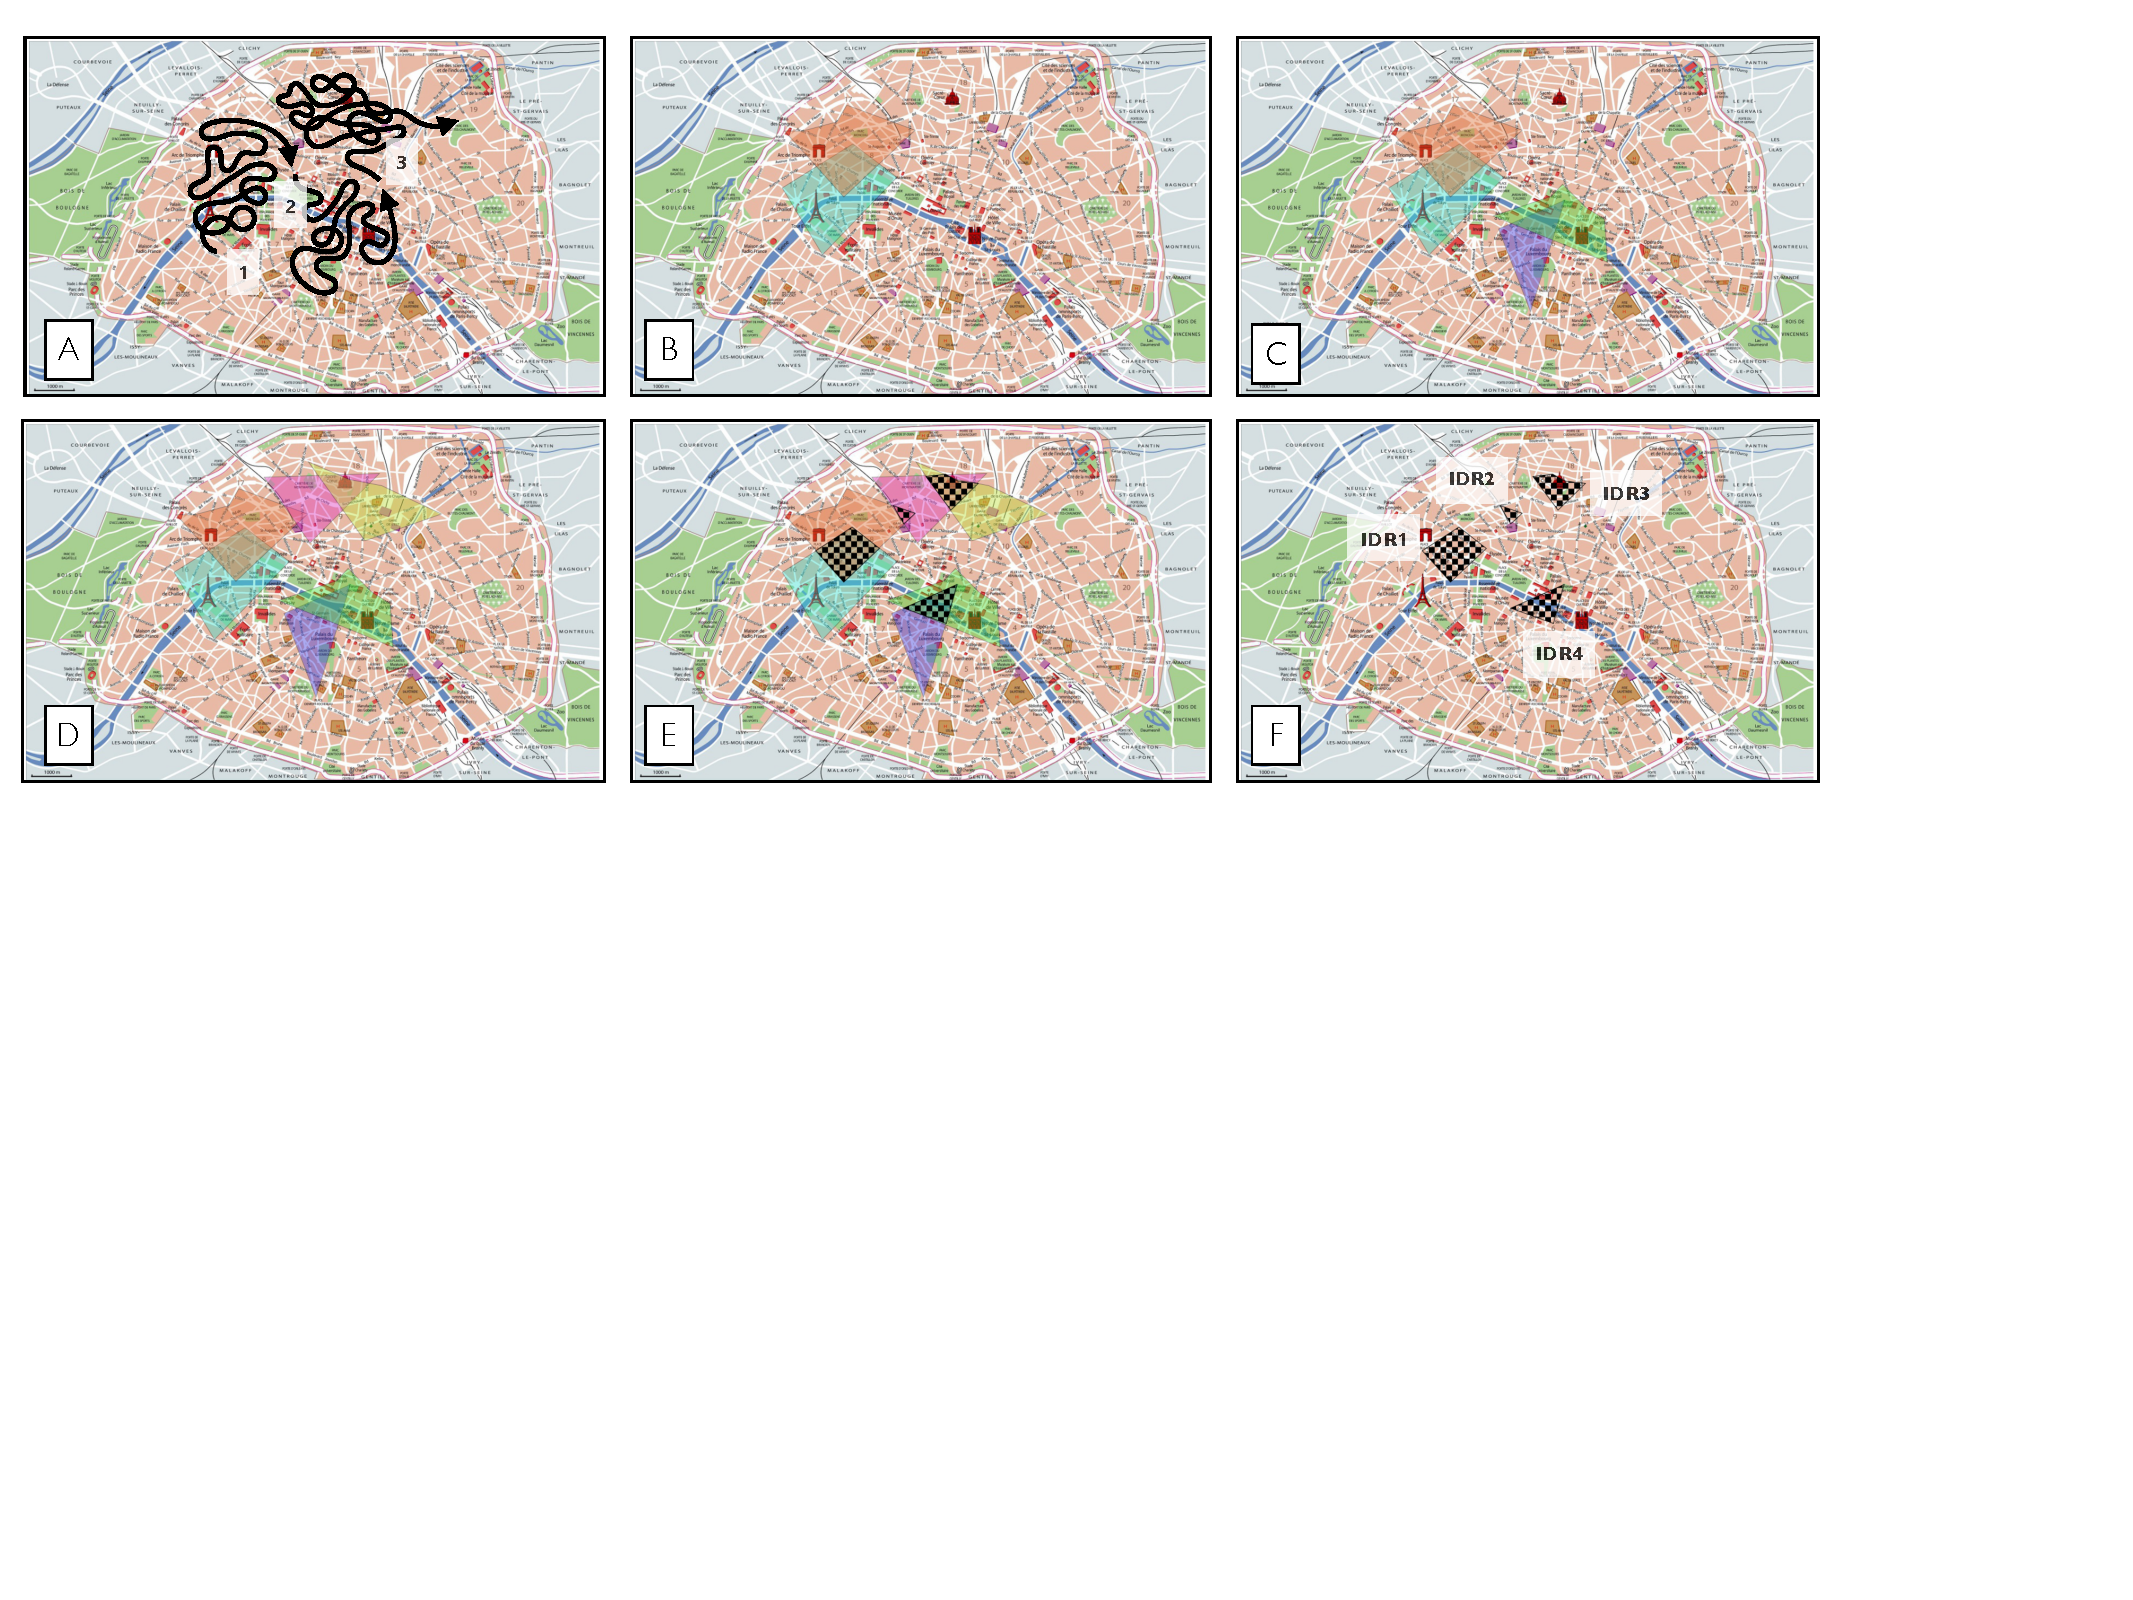
\includegraphics[width=\textwidth]{imgs/regions}
  \caption{The process of finding IDRs over Paris home-stays.}
  \label{fig:regions}
\end{figure*}

\begin{figure}[t]
\centering
   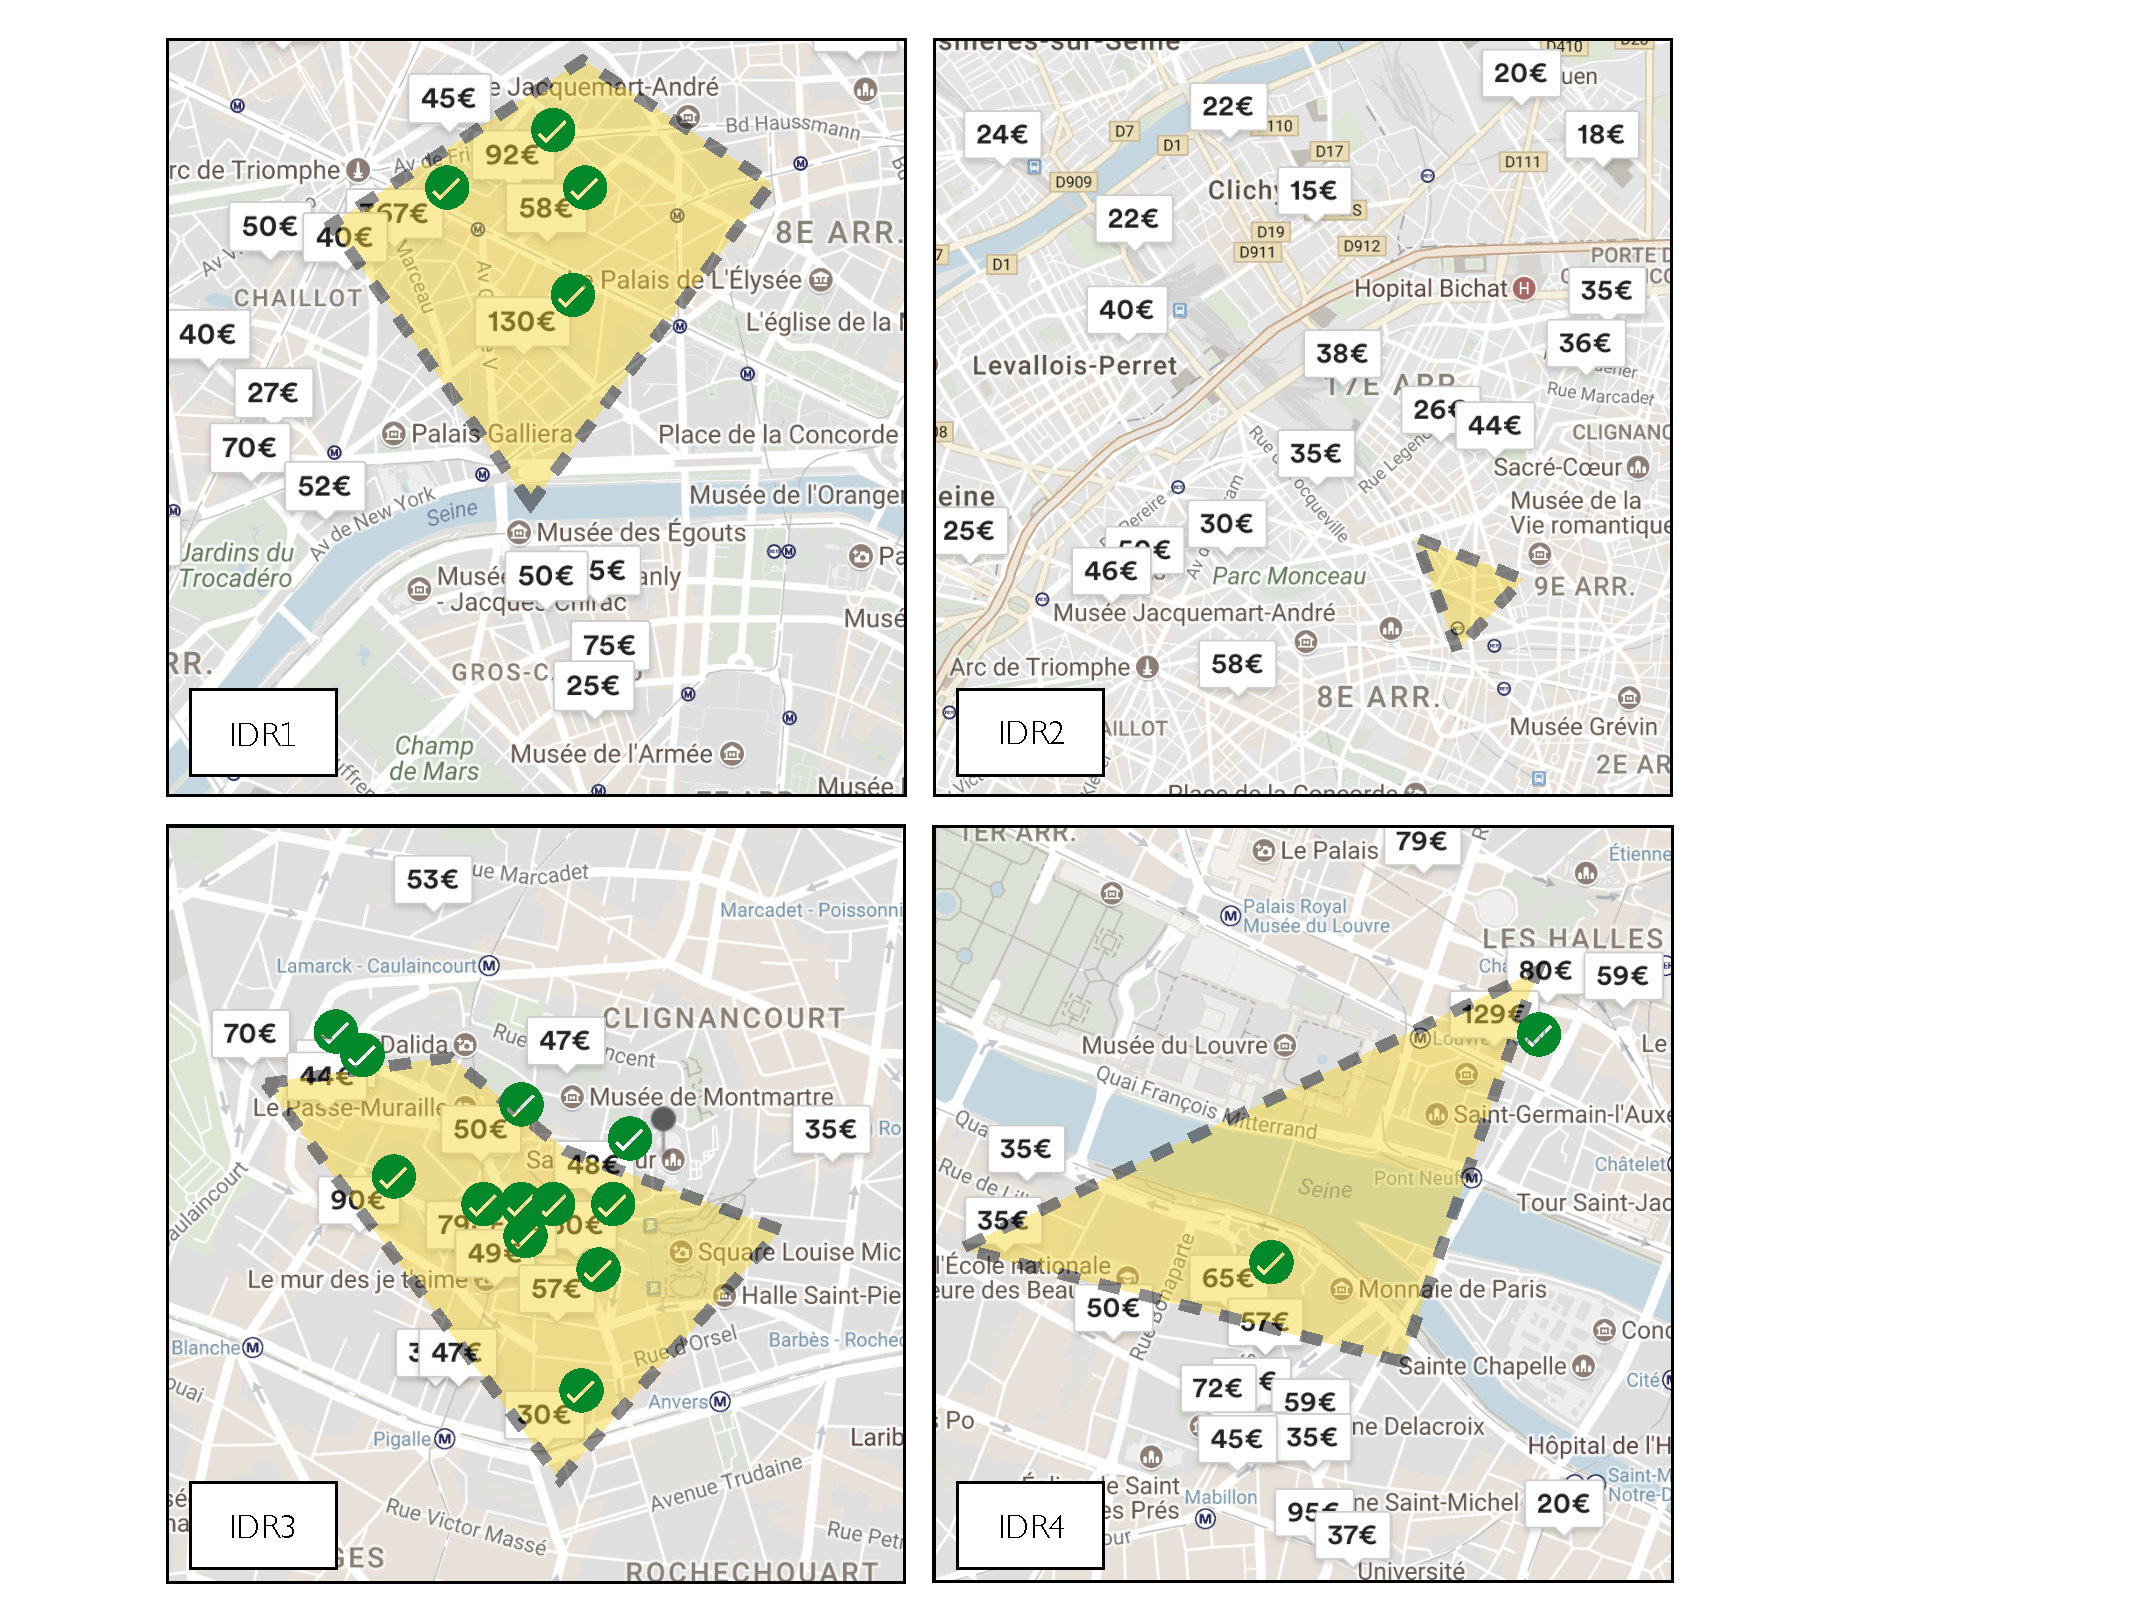
\includegraphics[width=\columnwidth]{imgs/match}
  \caption{Matching points for IDRs.}
  \label{fig:match}
\end{figure}

\vspace{2pt}
\noindent {\bf Example.} {\em Lucas is planning to spend few days in Paris, France. His appreciation of French culture makes him interested in new experiences in the city. He decides to rent a home-stay from Airbnb website\footnote{\it http://www.airbnb.com}. He likes to discover the city, hence he is open to any type of lodging in any region with an interest to stay in the city center. The website returns $4000$ different locations. As he has no other preferences, an exhaustive investigation needs scanning each location independently which is nearly infeasible. While he is scanning few first options, he shows interest in the region of ``Champ de Mars'' (near Eiffel Tower), but he forgets or doesn't feel necessary to click a point there. By discovering IDRs on his mouse moves over the home-stays in Paris, our system can quickly detect his interest in the region and short-list a small subset of locations (i.e., highlights) accordingly to be recommended to Lucas.}

\vspace{2pt}
We follow the above example to describe how IDRs are constructed in action.  Figure \ref{fig:regions} shows Lucas' steps to explore home-stays in Paris. Figure \ref{fig:regions}.A shows his mouse movements in different time stages. In this example, we consider $g = 3$ and capture Lucas' feedback in three different time segments (progressing from Figures \ref{fig:regions}.B to \ref{fig:regions}.D). It shows that Lucas started his search around Eiffel Tower and Arc de Triomphe (Figure \ref{fig:regions}.B) and gradually showed interest in south (Figure \ref{fig:regions}.C) and north (Figure \ref{fig:regions}.D) as well. All intersections between those clusters are discovered (hatching regions in Figure \ref{fig:regions}.E) which will constitute the set of IDRs (Figure \ref{fig:regions}.F), i.e., IDR1 to IDR4.

\vspace{2pt}
In the Airbnb dataset, points are home-stays. Figure \ref{fig:match} shows these points with their nightly price for IDRs. We observe that there exist many matching points with IDR3 and absolutely no matching point for IDR2. For IDR4, although there exist many home-stays below the region, we never check their containment, as they belong to a Quadtree cell which doesn't intersect with the IDR. 

\section{Experiments}
We discuss two sets of experiments. Our first set is on the usability of our approach. Then we focus more on discovering IDRs and present few statistics and insights for them. In the interest of space, we only present a glimpse of our experiments here. More will be presented in an extended report which we will make available upon acceptance. 

\vspace{2pt}
First off, we validate the ``usability'' of our approach. For this aim, we design a user study with some participants who are all students of Computer Science. Some of them are ``novice'' users who don't know the location under investigation, and some are ``experts.'' Participants should fulfill a task. For each participant, we report a variant of time-to-insight measure, i.e., how long the participants interact with the tool before fulfilling the task. Evidently, less number of interactions is preferred as it means that the participant can reach insights faster.

\vspace{2pt}
On the Airbnb dataset of Paris with 1,000 points, we define two different tasks: {\em T1: ``finding a point in a requested location''} (e.g., find a home-stay in the ``\textit{Champ de Mars}'' area), and {\em T2: ``finding a point with a requested profile''} (e.g., find a cheap home-stay.) Participants may also begin their navigation either from {\em I1: ``close to the goal''} or {\em I2: ``far from the goal''}. 


\begin{table}[h]
\centering
\caption{Interactions of ``novice'' and ``expert'' participants (in seconds)}
\label{tbl:novice}
\begin{tabular}{c|c|c|c|c|}
\cline{2-5}
                                       	& \textbf{T1/I1} 	& \textbf{T2/I1} 	& \textbf{T1/I2}	& \textbf{T2/I2}	\\ \hline
\multicolumn{1}{|c|}{Novices} 				& 1.99            	& 2.38	          	& 2.00              & 2.48              \\ \hline
\multicolumn{1}{|c|}{Experts} 				& 1.72            	& 2.09	          	& 1.70              & 2.14              \\ \hline
\end{tabular}
\end{table}


\vspace{2pt}
Table \ref{tbl:novice} shows the results. We observe that on average it takes $2.067$ seconds to achieve defined goal. This shows that implicit feedback capturing is an effective mechanism which helps analysts to reach their goals much faster. Expert participants need $0.35$ seconds less time on average. Interestingly, starting points, i.e., {\em I1} and {\em I2}, do not have a huge impact on number of steps. It is potentially due to the diversity component which provides distinct options and can quickly guide analyst towards their region of interest. We also observe that the task {\em T2} is an easier task than {\em T1}. This is potentially due to  where the analyst can request options similar to what she has already observed and greedily move to her preferred regions.

\vspace{2pt}
In the second part of our experiments, we employ two different datasets, i.e., Airbnb\footnote{\it \url{http://insideairbnb.com/get-the-data.html}} and Yelp\footnote{\it \url{https://www.yelp.com/dataset}}. We pick a similar subset from both datasets, i.e., home-stays and restaurants in Paris city, respectively. We consider four different sizes of those datasets, i.e., $100$, $1000$, $2000$ and $4000$ points, respectively. For each size of the datasets, we manually perform $20$ sessions, and then we present the results as the average of sessions.

\vspace{2pt}
We limit each session to $2$ minutes where we seek for interesting points in the datasets. We capture the following information in each session:

\begin{itemize}[leftmargin=*]
  \item The number of regions created from the mouse moves during the session;
  \item The number of generated IDRs (intersection of regions);
  \item The number of points from the dataset presented in each IDR;
  \item The coverage of points (in the dataset) with IDRs collectively.
\end{itemize}  

\vspace{2pt}
Tables \ref{tbl:airbnb} and \ref{tbl:yelp} show the result for Airbnb and Yelp, respectively. In Table \ref{tbl:airbnb}, we observe that the number of regions decreases when the number of points increases. On average, 10 regions are constructed per session. The average number of points presented in IDRs is $24.97$. It shows that our approach is able to highlight at least $8.05\%$ of points from the dataset, on average. 

\begin{table}[h]
\centering
\caption{IDR statistics on Airbnb dataset}
\label{tbl:airbnb}
\begin{tabular}{|c|c|c|c|c|}
\cline{1-5}
\textbf{\# points}  & \textbf{\# regions} 	& \textbf{\# IDRs} 	& \textbf{\# points in IDRs}	& \textbf{\%  points}	\\ \hline
\multicolumn{1}{|c|}{100} 				& 11.35            	& 10.05	          	& 29.40             & 29.40\%            
 \\ \hline
\multicolumn{1}{|c|}{1000} 				& 10.75          	& 6.75	          	& 11.70              & 1.17\%              \\ \hline
\multicolumn{1}{|c|}{2000} 				& 7.37           	& 3.63         	& 5.63             & 0.003\%              \\ \hline
\multicolumn{1}{|c|}{4000} 				& 10.30           	& 10.15	          	& 53.15              & 1.33\%              \\ \hline
\multicolumn{1}{|c|}{\textbf{average}} 				& \textbf{9.94}           	& \textbf{7.64}	          	&\textbf{ 25.97}              & \textbf{8.05\% }             \\ \hline

\end{tabular}
\end{table}

\vspace{2pt}
More uniform results are observed in Table \ref{tbl:yelp}, i.e., for Yelp dataset vis-\`a-vis Airbnb. The average number of generated regions reaches $12.75$ per session. Also,tThe number of regions decreases by increasing the number of points. The same happens for IDRs, where we obtain an average of $8.9$ IDRs generated per session. The number of points presented in IDRs is on average $108.65$ and it represents on average $13.11\%$ of points highlighted from the dataset.

% For both datasets we considered the location presented in our example scenario, where Lucas is planning to pass some vacations days in Paris. 

\begin{table}[h]
\centering
\caption{IDR statistics on Yelp dataset}
\label{tbl:yelp}
\begin{tabular}{|c|c|c|c|c|}
\cline{1-5}
\textbf{\# points}  & \textbf{\# regions} 	& \textbf{\# IDRs} 	& \textbf{\# points in IDRs}	& \textbf{\%  points}	\\ \hline
\multicolumn{1}{|c|}{100} 				& 14.90            	& 7.55	          	& 28.30             & 28.30\%            
 \\ \hline
\multicolumn{1}{|c|}{1000} 				& 13.90         	& 10.00	          	& 149.55             & 14.96\%              \\ \hline
\multicolumn{1}{|c|}{2000} 				& 11.05         	& 9.80         	& 111.05             & 5.55\%              \\ \hline
\multicolumn{1}{|c|}{4000} 				& 10.45          	& 8.55	          	& 145.7              & 3.64\%              \\ \hline
\multicolumn{1}{|c|}{\textbf{average}} 				& \textbf{12.57}           	& \textbf{8.97}	          	& \textbf{108.65}              & \textbf{13.11\%}              \\ \hline
\end{tabular}
\end{table}


\section{Conclusion}
In this paper, we present an approach to explore Interesting Dense Regions (IDRs) using implicit feedback in order to detect analyst latent preferences. The implicit feedbacks are captured from mouse moves of analysts over the geographical map while analyzing spatial data. We formalize a novel polygon-based mining algorithm which returns few highlights in line with analyst's implicit preferences. The highlights enable analysts to focus on what matters the most and prevent information overload.

\vspace{2pt}
We consider various directions of future work for this work. First, we are interested to incorporate an ``explainability'' component which can describe causalities behind preferences. For instance, we are interested to find seasonal patterns to see why the preferences of analysts change from place to place during various seasons of the year. Another direction is to incorporate ``Query by Visualization'' approaches, where analysts can specify their intents alongside their implicit preferences, directly on the map \cite{siddiqui2016effortless}.

\bibliographystyle{ACM-Reference-Format}
\bibliography{main}

\end{document}
